\documentclass{book}

\usepackage[margin=1in]{geometry}
\usepackage{amsmath,amssymb, amsthm}


\usepackage[backend=biber,
	style=alphabetic,
	%	citestyle=authoryear,
	natbib=true,
	url=true, 
	doi=true,
	eprint=false ]{biblatex}
	
	\addbibresource{../refs.bib}


\usepackage{color}
	\definecolor{deepgreen}{rgb}{0,0.5,0}

\usepackage[colorlinks=true, citecolor=deepgreen]{hyperref}

\usepackage{microtype}
\usepackage{tikz}
	\usetikzlibrary{positioning}\usetikzlibrary{arrows}
	\usetikzlibrary{shapes}
	\tikzset{every edge/.style={ % Sets the properties for each transition	1
			draw,
			->,
			auto,
			very thick}}
\usepackage{parskip}

\newtheorem*{remark}{Remark}


%%%%%%%%%%%%%%%%

\DeclareMathOperator*{\argmax}{arg\,max}
\DeclareMathOperator*{\argmin}{arg\,min}
\DeclareMathOperator*{\E}{\mathbb E}


\newcommand\Tstrut{\rule{0pt}{5.6ex}}         % = `top' strut
\newcommand\Bstrut{\rule[-0.9ex]{0pt}{0pt}}   % = `bottom' strut

\newcommand\geqc{\succcurlyeq}
\newcommand\leqc{\preccurlyeq}

\setlength{\skip\footins}{1cm}
\setlength{\footnotesep}{0.4cm}

\renewcommand*\thesection{\arabic{section}}

\begin{document}
	\chapter{Examples}
	
	\section{Wrong Variables.}
	Suppose worlds are parameterized by three variables $A, B, C$, each of which can take on two values: variable $A$ can take on either $a$ or $\bar a$, $B$ can take on $b$ or $\bar b$, and $C$ is either $c$ or $\bar c$.
	
	Suppose further that an agent cannot observe these variables directly, but rather observes variables $X$ and $Y$, which are logically defined as 
	\begin{align*}
		X &:= A \land B \\
		Y &:= B \lor C
	\end{align*}
	
	and that the agent originally has a preference order
	\[ x \bar y \geqc \bar x y \geqc \bar x \bar y \geqc x y  \]
	
	The variables $X$ and $Y$ are perfectly well-defined, and don't vary with time\footnote{which is already more than can be said for most variables that people care about --- for example, `nutritious', `inoffensive', and `affluent' are all moving targets}, and yet still there is a good reason for the agent, upon discovering the true nature of the world, to change its preferences. Below is a table of which assignments of the $XY$ variables correspond to the $ABC$ variables:
	
	
	
	\begin{center}
		\begin{tabular}{cccc}
			$x \bar y $ & $\bar x y$ & $\bar x \bar y$ & $x y$ \\\hline
			\rule{0pt}{2.3em}$\varnothing$ & \parbox[c]{0.5cm}{$\bar a b \bar c$\\$\bar a b c$ \\ $a \bar b c$} 
				& \parbox[c]{0.5cm}{$\bar a \bar b \bar c$ \\ $a \bar b \bar c$}
				& \parbox[c]{0.5cm}{$abc$} \\[1.3em]\hline
		\end{tabular}
	\end{center}
	\vspace{1em}
	
	
	Now, imagine that you now discover the true nature of the world: its complete parameterization by $A,B,C$. There are two competing intuitions one might have about the right way to think about preferences.
	
	\subsubsection*{Type-level preferences as primitive}
	The first, and the one that jives best with the utility-maximization perspective, is that even seeing the world from this new perspective, your preferences really ought to be thought of as over the variables you observe ($X$ and $Y$). After all, discovering that you have actually been referring to many chemically distinct solutions as ``water'' (perhaps H$_2$O with various levels of fluoride and magnesium) should not necessarily cause you to disassociate them (maybe you can't even tell them apart!), let alone form separate value judgments towards every possible solution.
	
	In this interpretation, if the preference order above was truly what you had preferences for (and not merely that you were mistaken about what you enjoyed), then it does not matter what you discover about the world --- as far as you are concerned, the utility of a world parameterized by $A,B,C$ is determined purely by its effect on $X$ and $Y$. 
	
	This results in the following total pre-order (where the agent is indifferent to alternatives in the brackets):
	
	\[ \left\{~\parbox[c]{0.5cm}{$\bar a b \bar c$\\$\bar a b c$ \\ $a \bar b c$}~\right\} \geqc \left\{~\parbox[c]{0.5cm}{$\bar a \bar b \bar c$ \\ $a \bar b \bar c$}~\right\} \geqc \left\{abc \right\} \]
	
	The second intuition that one might have, is that you have been blind to the differences between certain worlds and have accidentally been conflating them. This treatment of type-level preferences as primitive is related to the ``top-down'' approach to relating type and token preferences, as in \cite[chapter 4, pg 55]{girard2008modal}
	
	\subsubsection*{Token-level preferences as primitive}
	
	The second intuition is that the broad, type-level preferences were merely an oversimplified expression of your past experiences. After all, you had to form your preferences somehow, and maybe there is a reason that you think  $\bar x y \geqc \bar x \bar y$.
	
	Suppose further that almost every experience you have with $\bar x y$ was in fact due to the world configuration $\bar a b \bar c$, and similarly, that most of your observations of $\bar x \bar y$ were due to the world being in state $\bar a \bar b \bar c$. In this case, it is reasonable to conclude, that by preferring $\bar x y$ to $\bar x \bar y$, really you are 
	
	
	\section{New Constraint}
	
	\section{Gamification}
	Gamification induce some intrinsic value into 
	
	From one perspective, this is an obvious part of the application of expected utility for decision making --- it is common for modelers to say things along the lines of ``by playing this game, I will get a(n expected) payoff of $g$ utils'', in the same sense that one would gain utility by watching a film or spending time with friends; these are simply regarded as atomic pleasure generation units.
	
	Still, 
	
	\section{Value Capture}
	
	
	\section{Cultural Revolution}
	
	%\section{Pure Mathematics}
	
	\chapter{The Model}
	\section{Notation}
	
	\begin{tabular}{r|l}
		$\Delta(X)$ & The set of distributions on a measurable set $X$ \\
		$\prod_{a : A} B(a)$ & A pi-type, or dependent product $B(a)$ whose type depends on the value of its input. 
	\end{tabular}
	
	\section{Formalism}
	
	
	We would like to describe preference dynamics on some set $X$ of alternatives. To this end, there are three pieces of formalism that we require: preference domains $\cal X$, beliefs $\mathcal B$ relating the domains, and a weighting of domains $W$.
	
	Let $\cal X$ be some collection of measurable pre-orders (sets which admit probability distributions, with transitive, reflexive relations). These are thought of as relevant representations, whose relations are (possibly empty) preference relations on their items. 
	
	Some subset of pairs of $\cal X$ are connected with beliefs about how the pairs are connected. Formally, this takes the form of a dependent product, 
	\[ \mathcal B : \prod_{X_1, X_2 : \mathcal X}  X_1 \to \Delta(X_2) \cup \{ \ast \}  \]
	Given domains $X_1$, $X_2$ from $\cal X$, $\mathcal B(X_1,X_2)$ is either empty ($\ast$), or a function from values in $X_1$ to distributions over $X_2$ --- or equivalently, a (possibly missing) conditional distribution $\Pr(X_2 | X_1)$.
%	\footnote{Note that this endows $\cal X$ itself with a pre-order}

	The final part of the formalism is a weighting $W : \cal X \to \mathbb{R}$ describing one's attachment to the ordering in each domain. When there is conflict, this weighting is used to figure out which preferences to revise.
	
	\[ D :  \]

	
	Without any additional assumptions, there is plenty of room for irrationality in this framework: for instance, we have not yet enforced that compositions of these probability distributions marginalize out properly.
	
	
	
	We can think of preferences flowing along $\cal B$. Note that if $\mathcal B$ is acyclic, this means that the ``source'' nodes are static preferences. Accounts of preference change that relegate preference change to these \footnote{This is similar to the first kind of preference dynamics \cite{grune2009preference}, appealing to some more primitive construction which already is endowed with some ordering and. Examples include property weightings \cite{dietrich2013preferences} and preference bases \cite{girard2008modal}} 
	

	\section{Examples}
	\subsection{Framing Effects}
	Suppose we are offered a choice between alternatives in $X$, described in two different ways. Standard theories have difficulty even representing this state of affairs for agents, but here we can set $\mathcal X = \{ X, X'\}$. 
	
	At first, we have preferences $x \leqc_X y$, and $x' \geqc_Y y'$. As an external observer, this seems crazy, because we have a degenerate belief distribution which exactly identifies $x$ and $x'$ --- but at first perhaps our agent either has not thought about how the two domains connect before, or has some uncertainty about exactly how strong this connection is.
	
	As the agent assures herself that the correspondence is in fact perfect, the beliefs approach a perfect correspondence, creating cognitive dissonance. As the belief revision may be incredibly expensive, the agent is pressured into either changing her preferences on $X$ or $X'$.
	
	\subsection{Music Preferences}
	We will select four domains $\mathcal X = \{ X, S, A, G\}$. $X$ is the set of actual instantiations of a song being played (which uniquely determine the time, context, mood, memory of the agent, and so on). $S$ is the set of songs, $A$ is the set of artists, and $G$ is the set of genres. $\cal B$ is the degenerate distribution which deteriministically picks out the song being played, and its artist and genre, as illustrated graphically below:
	
	\begin{center}
		\itshape
		\color{blue}
		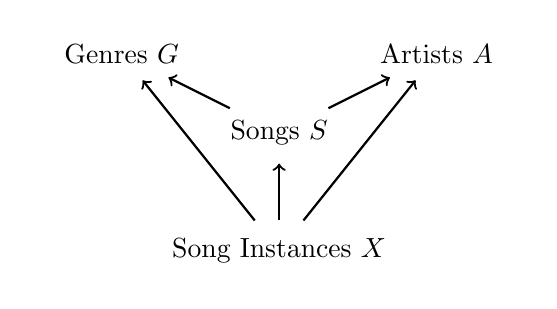
\begin{tikzpicture}
			\node[ellipse] (A) at (2,2) {Artists $A$};
			\node[ellipse] (G) at (-2,2) {Genres $G$};
			\node[ellipse] (S) at (0,1) {Songs $S$};
			\node[ellipse] (X) at (0,-0.5) {Song Instances $X$};
			
			\draw[->, thick] (X) -- (S);
			\draw[->, thick] (S) -- (A);
			\draw[->, thick] (S) -- (G);
			\draw[->, thick] (X) -- (A);
			\draw[->, thick] (X) -- (G);
		\end{tikzpicture}
	\end{center}
	
	One can independently have preferences over each of these sets, but there are clearly ways that they could be in conflict: for instance, if you prefer every instance of song $s$ to every instance of song $t$, then it would seem wrong to also prefer $t$ to $s$ in the song domain.  We use this conflict to model cognitive dissonance, and motivate preference changes.
	
	For instance, 
	
	\subsection{Meta-preferences as Exponentials}
	If $X$ is a preference domain, one can also form a preference domain $\mathfrak M_X$ consisting of preferences. Combined with the belief 
	
	
	\subsection{Non-transtive Preferences}
	One might take issue with the fact that different scales of belief revision may require
	
%	You, however, not being able to observe the world, have preferences for $C := A \otimes B$, for $D := B \otimes C$, and also for $E := C \otimes A$, amounting to a choice of exactly one out of every pair of real variable. All three conjunctions are, of course, unsatisfiable.

	\chapter{A Theory of Preferences}
	
	The general idea is as follows: rather than thinking of preferences as uniform objects, we want to discriminate between preferences which are expressed in different ways. In particular, some propositions are more concrete than others, and some are more actionable than others, which results in very different effects when an agent experiences a distributional shift. For instance, if an agent only has preferences over actions (or policies), independent of the states of the world, then very little computation is required to infer a policy. If the agents' most closely-held preferences are expressed in this form, then there is no need for planning, or sub-goals --- which is to say, there are no downstream tasks. At the other extreme, we can also specify an agent's preferences succinctly in terms a single final goal, from which one can do planning, but admits no further compression.
	
	
	
	This is a very silly, not-particularly-agentive agent, but if instead we had preferences over policies (which is equally grounded), then we are simply modeling the external behavior of an agent directly. Given an unbounded number of samples and a way to ``reset'' an agent, the policy (or policies) that the agent acts by could be recorded. 
	
	Savage takes one possible first step down this compression network, and shows that (under certain rationality assumptions) a preference over policies induces both a utility function over state/action pairs, and a probability distribution over states, with which the agent's behavior is captured by expected utility maximization.
	
	%TODO: show this more carefully.
	
	
	To each proposition $\varphi$, we can speak of an agents' belief $\Pr\varphi$ that $\phi$ the agent's utility $U \varphi$ of $\varphi$, and also 
	
 	At the very lowest level, a preference over 
	
	
	Let $\mathcal W$ be the set of world states, and $\mathsf A_w$ be the set of actions that can be taken in world $w \in \mathcal W$. Then a policy $\pi : \prod_{w: \mathcal W} \mathsf A_w$ is a function which returns a variable action
	

	
	
	For simplicity, we will represent preferences as utilities. For every language $\Lambda$, one can assume a utility function $U : \Lambda \to \mathbb R$, which assigns a utility to a given formula. 
	
	A policy
		\[ \pi: \mathrm{States} \to \mathrm{Actions} \]
	
	
	
	\section{The Stream}

	\chapter{Context}
	From a a modeling perspective, what can be said to determine [a person]'s actions? Why do [people] do things? These are some of the central questions in behavioral economics. 
	
	
%	\begin{center}\scshape\color{blue}\selectfont
%		\begin{tikzpicture}[align=center]
%			\node (O) {Order \\ Coffee};
%			\node [right=2em of O] (C) {Drink \\ Coffee};
%			\node [right=2em of C] (W) {Work more \\effectively};	
%			\node [above right=1em of W] (A) {Not Disappointing\\ Advisor};
%			\node [right=2em of W] (I) {Work is Valuable};
%			
%			\draw (O) edge (C) (C) edge (W) (W) edge (A) (W) edge (I);
%		\end{tikzpicture}
%	\end{center}
	
	The chain of rational reasons then bottoms out with some desire, moral, preference, which is not itself the kind of thing that can be interrogated with the question ``why'', in the same way. Sure, there may be a causal explanation for why it came to be that you enjoy coffee, but that is not the 
	
	
			
	
%	If $S$ is a set of states, and $O$ is the set of outcomes, 
	
%	let $\mathcal L$
	
	% By Savage, we know that we don't need to assumsemithicke the existence of a probability distribution (over states or outcomes); one can derrive this from the axioms
	
	\section{The Emotion / Reason Dichotomy}
	Morals, preferences, goals, utilities, rewards/punishments, and desires all have something in common: the behavior that characterizes them is an optimization. They answer a question about \emph{why} something was done, in a way that is compatible with planning and rational, well-thought-out behavior. If one sees a person repeatedly doing something, say walking their dog, it is reasonable to conclude that either they hold that this is a morally good thing to do, have a preference or goal / sub-goal of walking their dog, enjoy it, or have times when they want to do it. Moreover, these are considered explanations of \emph{why} behavior happens. They are descriptions of the things that agents optimize.
	
	The second feature they share is a subjectivity: anyone can have any preferences or utilities or rewards (perhaps subject to certain constraints if you don't want to be manipulated, want to behave robustly in the presence of adversaries, and so on). Once the space has been constrained, having different preferences is merely... a matter of preference. The theories we use for modeling agents do not take into account the mechanisms by which one might obtain preferences, which 
	
	More egregiously still, standard utility / reward maximization picture has nothing to say about the possibility of these quantities changing over time.
	
	
	
	All of this is to be contrasted with two other concepts:

	\begin{enumerate}
		\item Empirical analysis which determines that some behavior (as opposed to another one) is occurring. 
		\item Theories of belief, rationality, and \emph{how} to optimize.
	\end{enumerate}
	
	
	
	All of these have been postulated as reasons why people do things, and more generally, as theories about ways to shape behavior of agents. 
	
	
	
	The general idea is to consider two descriptions of motivation equivalent if they necessarily result in indistinguishable behavior. 
	
	% Related: opinions --- beliefs + judgement
	% 	Emotions --- attitudes towards things [mroe general]
	
	\subsection{Utilities and Preferences}
	
	To simplify things, economists and decision theorists start with the case when the set of possibilities is small and finite. If $O$ is the set of things one could choose between, i.e., the set of outcomes, then we can formalize a preference as a pre-order $(O, \preccurlyeq)$ on $O$.
	
	\begin{align*}
		\forall x \in O.&~x \preccurlyeq x \tag{Reflexivity}\\
		\forall x,y,z \in O.&~(x\preccurlyeq y)~\land~( y \preccurlyeq z) \Rightarrow~(x \preccurlyeq z) \tag{Transitivity}
	\end{align*}
	
	Rather than dealing with the partial order directly, we might like to have an embedding into something we have more intuition for, such as natural numbers or a continuous space. The problem with this, of course, is that the space may have some structure which is incompatible with the partial order. 
	
	of these results in a ranking, 
	
	However, there is often a lot more structure on outcomes
	
	
	

	
	\subsection{Utilities and Rewards}
	
	Both utilities and rewards are real-valued functions from something in the world to a one-dimensional notion of `good-ness' represented by $\mathbb R$, and hence are sometimes thought of as equivalent; here we will do some of the work to explore in what sense they might be equivalent, and the sorts of issues that might come up if conflating the two without any thought.
	
	Utilities are over outcomes, so a utility function $U : Z \to \mathbb R$ must be
	
	\[ \pi^*(x) = \argmax_{y: Y} \E_{z : Z} \Big[ U(z)~\Big|~ y,x\Big] \]
	
	\subsubsection{Determinism}
	If $\cal W$ is the set of all possible world states, and $\tau: \cal W \to W$ is a deterministic function describing the evolution of the world, then having a preference over futures starting at $w_0$ and consistent with $\tau$ is meaningless, as there is only one such sequence of worlds. Therefore, pure determinism only makes sense with agents with imperfect information. 
	
	Let $X$ be the space of world representations for an agent, and let $\eta: \mathcal W \to X$ be some function, thought of as perception, which generates a world representation. This gives us an equivalence class $[w] := \eta^{-1}(\eta(w))$ of information sets of the agent, which may not be stable under $\tau$, and so it may be the case that $w \underset\eta\sim w'$ but not $\tau(w) \underset\eta\sim \tau(w')$
	
	
	
	The fact that one gets more information over time suggests that the optimal policy, even with infinite computation, in general will change with additional samples. After two steps, the policy becomes
	
	\begin{align*}
		\pi^*(\eta\circ\tau (x)) &= \argmax_{y: Y} \E_{z : Z} \Big[ U(z)~\Big|~ y,\eta\tau x \Big]  \\
			&= \argmax_{y: Y} \int\limits_{\mathrm dZ} \Pr\Big[z~\Big|~\left(Y^{(t)} = y \right) \land \left(X^{(t)}= \eta \circ \tau (x)\right) \land \left(X^{(t-1)} = x \right) \Big] U(z)
	\end{align*}
		
	
	\subsubsection{Nondeterminism}
	Once again, suppose $\cal W$ is the set of possible worlds, with now $\tau: \mathcal W \to 2^{\mathcal W}$, a non-deterministic version of the transition function in the deterministic setting from before.
	
	In this more general case, we can still relate the two. To begin, suppose that we have a complete preferences over possible futures. 
	
	
	\section{Related Problems in Other Fields}
	
%	\subsection{Selective Pressure}
	\subsection{Art History} % Model literally changes in peoples' aesthetic preferences
	\subsection{Pedagogy} % Representation Changes.
	\subsection{}
	
	
	\section{Applications}
	
	\subsection{Content Recommendation}
	The way that these assumptions of static preferences manifest themselves in content recommendation systems is the
	
	\subsection{AI Safety}
	\subsection{Better Inverse Reinforcement Learning}
	\subsection{Robotics: Life-long Learning}
	\subsection{Meta Ethics}
	
	\section{As a Learning Problem}
	
	\nocite{*}
%	\printbibliography
	
	
\end{document}